\documentclass{article}
\usepackage{amsmath, amssymb}
\usepackage{pgfplots}
\usepackage{listings}
\usepackage{mathwriteup}

\begin{document}

% Set the context for this problem - this information appears in the page header
% and helps the hint system understand what material you've covered
\mathwriteupcontext{
  author=Keith Murray,
  assignment=Homework 3,
  disclosure=Generative AI was used\\ Collaborated with Jeremy S. and Sasha L.
}

\begin{problem}
Consider the equations of motion for the simple pendulum with linear damping $\delta$ and constant applied torque $\beta$:
\[ \ddot{\theta}+\delta\dot{\theta}+\sin\theta=\beta \]
where $\delta,\beta\geq 0$ and $\theta$ is on the circle $S^1$ (which can be identified with the interval $[-\pi,\pi)$).
\begin{enumerate}
  \item[(a)] Find conditions on $(\beta,\delta)$ for which fixed points exist, linearize at the fixed points and draw conclusions on their stability types. Allow the parameters $(\beta,\delta)$ to vary, and locate values for which the linearizations are degenerate (non-hyperbolic).
  \item[(b)] For $\delta=0$, there is a conserved quantity (the system is Hamiltonian). Use this to deduce global phase portraits, and compare with information from (a).
  \item[(c)] For $\delta>0$, can this system have closed orbits that \textbf{do not} encircle the `phase cylinder'? [\textit{Hint:} Use Bendixson's criterion.]
  \item[(d)] For $\delta>0$ and $\beta>0$, can the system have closed orbits that \textbf{do} encircle the phase cylinder? [\textit{Hint:} Determine a trapping region and apply the Poincare-Bendixson theorem.]
\end{enumerate}

\end{problem}

\begin{solution}
\section{Problem 1}
\subsection{Part (a)}
Let's first rewrite our system into a two system ODE:
\begin{align*}
  \dot{\theta}&= \omega\\
  \dot{\omega}&= \beta -\delta \omega -\sin\theta
\end{align*}
To find fixed points, we can set these equations equal to 0:
\begin{align*}
  \dot{\theta}&= 0\\
  \dot{\omega}&=0= \beta -\delta \omega -\sin\theta=\beta -\delta \cdot 0 -\sin\theta
\end{align*}
Hence we have fixed points when
\[ \sin\theta = \beta \]
We can think about the number of fixed points and their positions as a horizontal line that starts at $\beta=0$ and then sweeps to $\beta=+1$:
\begin{itemize}
  \item $\beta= 0$ --- There are two fixed points with one at $\theta=-\pi$ and the other in at $\theta=0$.
  \item $0<\beta\leq 1$ --- There are two fixed points with one in the range $\theta\in(0, \pi / 2)$ and the other in the range $\theta\in(\pi / 2, \pi)$. Note that because of the boundary condition of $S^1$, the fixed point in $\theta\in(\pi / 2, \pi)$ is a ``continuation'' of the fixed point previously from $\theta=-\pi,$.
  \item $\beta=1$ --- There is one fixed point at $\theta=\arcsin(-1)=\frac{\pi}{2}$
\end{itemize}
To be explicit, we can write the fixed points $(\theta,\omega)$ as the following
\begin{itemize}
  \item $\beta=0$ gives us $(-\pi,0),(0,0)$
  \item $0<\beta\leq 1$ gives us $\left(\arcsin\beta,0\right),(\pi-\arcsin\beta,0)$
  \item $\beta=1$ gives us $(\frac{\pi}{2},0)$
\end{itemize}
Note that we have to add the $\pm\pi$ values to the fixed points when $|\beta|<1$ because $\arcsin$ is only defined for $|x|\leq 1$ . Now let's linearize around each fixed point to determine their stability. 

To linearize, we can compute the Jacobian 
\[ J_f(x,y) = \begin{bmatrix}
\frac{\partial f_1}{\partial \theta} & \frac{\partial f_1}{\partial \omega} \\
\frac{\partial f_2}{\partial \theta} & \frac{\partial f_2}{\partial \omega} 
\end{bmatrix} \]
with the quantities being 
\begin{gather*}
  \frac{\partial f_1}{\partial \theta}=0\\
  \frac{\partial f_1}{\partial \omega}=1\\
  \frac{\partial f_2}{\partial \theta}=-\cos\theta\\
  \frac{\partial f_2}{\partial \omega}=-\delta
\end{gather*}

Before we focus on fixed points, let's note some useful expressions:
\[
\cos\left(\arcsin \beta\right)=\sqrt{1-\sin\left(\arcsin\beta\right)^2}=\sqrt{1-\beta^2}
\]
For $\cos\left(\pm\pi-\arccos\beta\right)$, the expression is a bit more complicated, but we can make use of the identity $\cos(t-s)=\cos t \cos s + \sin t \cos s$:
\begin{align*}
  \cos\left(\pm\pi-\arccos\beta\right)&=\cos \left(\pm \pi\right) \cos\left(\arccos\beta\right) + \sin \left(\pm \pi\right) \cos \left(\arccos\beta\right)\\
  &=-1\cdot \cos\left(\arccos\beta\right)+0\cdot \cos \left(\arccos\beta\right)\\
  &=-\sqrt{1-\beta^2}
\end{align*}

Now dealing with the case of $\beta=0$, we can start with the fixed point $(0,0)$. The Jacobian is 
\[ Df(0,0) = \begin{bmatrix}
0 & 1 \\
-1 & -\delta
\end{bmatrix} \]
Via SymPy, we get the following eigenvalues
\[
\lambda_0 = - \frac{\delta}{2} - \frac{\sqrt{\delta^2 - 4}}{2}, \qquad \lambda_1 = - \frac{\delta}{2} + \frac{\sqrt{\delta^2 - 4}}{2}
\]
where we have three cases: (1) $\delta=0$, (2) $0<\delta<2$, (3) $\delta\geq2$.
\begin{enumerate}
  \item For $\delta=0$, both eigenvalues become $\lambda_0=-i,\lambda_1=+i$ and linearization tells us nothing. The fixed point is non-hyperbolic.
  \item For $0<\delta<2$, both eigenvalues are complex with negative real parts. Hence, $(0,0)$ is stable. In particular, it is a stable spiral.
  \item For $\delta\geq2$, both eigenvalues are real and negative. Note that $\lambda>\sqrt{\lambda^2-4}$ so $\lambda_1$ is indeed negative. Therefore, $(0,0)$ is stable. In particular, it is a stable node.
\end{enumerate}

Now continuing with $\beta=0$, we can move to the fixed point $(-\pi,0)$. The Jacobian is 
\[ Df(0,0) = \begin{bmatrix}
0 & 1 \\
1 & -\delta
\end{bmatrix} \]
Via SymPy, we get the following eigenvalues
\[
\lambda_0 = - \frac{\delta}{2} - \frac{\sqrt{\delta^{2} + 4}}{2}, \qquad \lambda_1 = - \frac{\delta}{2} + \frac{\sqrt{\delta^{2} + 4}}{2}
\]
where for all values of $\delta$, it follows that $\lambda_0$ is negative and $\lambda_1$ is positive (note that $\delta<\sqrt{\delta^2+4}$). Hence, $(-\pi,0)$ is a saddle.

Now dealing with the case of $0<\beta\leq 1$, we can start with the fixed point $\left(\arcsin\beta,0\right)$. The Jacobian is 
\[
Df\left(\arcsin\beta,0\right)=\begin{bmatrix}
0 & 1 \\
-\cos\left(\arcsin\beta\right) & -\delta
\end{bmatrix} = \begin{bmatrix}
0 & 1 \\
-\sqrt{1-\beta^2} & -\delta
\end{bmatrix}
\]
Via SymPy, we get the following eigenvalues and eigenvectors
\[
\left(\lambda_0= - \frac{\delta}{2} - \frac{\sqrt{\delta^{2} - 4 \sqrt{1 - \beta^{2}}}}{2}, \ v_0=   \left[\begin{matrix}- \frac{\delta}{\sqrt{1 - \beta^{2}}} - \frac{\lambda_0}{\sqrt{1 - \beta^{2}}}\\1\end{matrix}\right]\right)
\]
and 
\[
 \left(\lambda_1= - \frac{\delta}{2} + \frac{\sqrt{\delta^{2} - 4 \sqrt{1 - \beta^{2}}}}{2}, \  v_1= \left[\begin{matrix}- \frac{\delta}{\sqrt{1 - \beta^{2}}} - \frac{\lambda_1}{\sqrt{1 - \beta^{2}}}\\1\end{matrix}\right]\right)
\]
Examining our eigenvalues, we only care about the sign of 
\[-\delta - \sqrt{\delta^{2} - 4 \sqrt{1 - \beta^{2}}}\qquad\text{and}\qquad -\delta + \sqrt{\delta^{2} - 4 \sqrt{1 - \beta^{2}}}\]
We have two cases: (1) $\delta=0$ and linearization fails due to purely imaginary eigenvalues, (2) the term $\sqrt{\delta^{2} - 4 \sqrt{1 - \beta^{2}}}$ is real and (3) the term $\sqrt{\delta^{2} - 4 \sqrt{1 - \beta^{2}}}$ is imaginary. In the case of (2), it necessarily follows that
\[\delta^2 > \delta^{2} - 4 \sqrt{1 - \beta^{2}},\]
hence we can state that $-\delta - \sqrt{\delta^{2} - 4 \sqrt{1 - \beta^{2}}}$ and $-\delta + \sqrt{\delta^{2} - 4 \sqrt{1 - \beta^{2}}}$ both have negative real parts, implying that $\left(\arcsin\beta,0\right)$ is a stable node. In the case of (3), it follows that $-\delta - \sqrt{\delta^{2} - 4 \sqrt{1 - \beta^{2}}}$ and $-\delta + \sqrt{\delta^{2} - 4 \sqrt{1 - \beta^{2}}}$ both have negative real parts, implying that $\left(\arcsin\beta,0\right)$ is a stable spiral. In fact, it is the value of $\delta$ that determines whether $\left(\arcsin\beta,0\right)$ is a stable spiral or stable node:
\begin{itemize}
  \item For $\delta^2 \geq 4 \sqrt{1 - \beta^{2}}$, we have a stable node 
  \item For $\delta^2 < 4 \sqrt{1 - \beta^{2}}$, we have a stable spiral
  \item For $\delta=0$, we have purely imaginary eigenvalues and linearization fails. The fixed point is non-hyperbolic.
\end{itemize}

For our fixed point $\left(\pi - \arcsin\beta,0\right)$, the Jacobian is 
\[
Df\left(\pi - \arcsin\beta,0\right)=\begin{bmatrix}
0 & 1 \\
-\cos\left(\pi - \arcsin\beta\right) & -\delta
\end{bmatrix} = \begin{bmatrix}
0 & 1 \\
\sqrt{1-\beta^2} & -\delta
\end{bmatrix}
\]
Via SymPy, we get the following eigenvalues and eigenvectors
\[
\left(\lambda_0= - \frac{\delta}{2} - \frac{\sqrt{\delta^{2} + 4 \sqrt{1 - \beta^{2}}}}{2}, \ v_0=   \left[\begin{matrix}- \frac{\delta}{\sqrt{1 - \beta^{2}}} - \frac{\lambda_0}{\sqrt{1 - \beta^{2}}}\\1\end{matrix}\right]\right)
\]
and 
\[
 \left(\lambda_1= - \frac{\delta}{2} + \frac{\sqrt{\delta^{2} + 4 \sqrt{1 - \beta^{2}}}}{2}, \  v_1= \left[\begin{matrix}- \frac{\delta}{\sqrt{1 - \beta^{2}}} - \frac{\lambda_1}{\sqrt{1 - \beta^{2}}}\\1\end{matrix}\right]\right)
\]
Examining our eigenvalues, we only care about the sign of 
\[-\delta - \sqrt{\delta^{2} + 4 \sqrt{1 - \beta^{2}}}\qquad\text{and}\qquad -\delta + \sqrt{\delta^{2} + 4 \sqrt{1 - \beta^{2}}}\]
It clearly follows that $-\delta - \sqrt{\delta^{2} + 4 \sqrt{1 - \beta^{2}}}$ is a negative real number, and that 
\[\delta^2 < \delta^{2} + 4 \sqrt{1 - \beta^{2}},\]
hence $-\delta + \sqrt{\delta^{2} + 4 \sqrt{1 - \beta^{2}}}$ is a real positive number. Therefore, it follows that $\left(\pi - \arcsin\beta,0\right)$ is a saddle for all values of $\delta$.

For the case of $\beta=1$, we have 
\[
Df\left(\frac{\pi}{2},0\right)=\begin{bmatrix}
0 & 1 \\
-\cos\left(\frac{\pi}{2}\right) & -\delta
\end{bmatrix} = \begin{bmatrix}
0 & 1 \\
0 & -\delta
\end{bmatrix}
\]
For the eigenvalues and eigenvectors, we have 
\[
\left[ \left( \lambda_0 = 0, \  v_0=\left[ \left[\begin{matrix}1\\0\end{matrix}\right]\right]\right), \  \left( \lambda_1 = - \delta, \  v_1=\left[ \left[\begin{matrix}- \frac{1}{\delta}\\1\end{matrix}\right]\right]\right)\right]
\]
where a $\lambda_0 = 0$ tells us that this fixed-point is degenerate (non-hyperbolic).

\subsection{Part (b)}

To show that our system is Hamiltonian, we have to show there is a function $H(x,y)$ such that
\begin{align*}
  \dot{\theta}&=\frac{\partial H}{\partial \omega}\\
  \dot{\omega}&=-\frac{\partial H}{\partial \theta}.
\end{align*}
Starting with $\dot{\theta}$, we can write 
\begin{gather*}
  \frac{\partial H}{\partial \omega}=\omega\\
  \partial H=\omega\partial \omega\\
  \int \partial H = \int \omega\partial \omega\\
  H(\theta,\omega)=\frac{\omega^2}{2}+f(\theta)
\end{gather*}
Moving on to $\dot{\omega}$, we can write 
\begin{gather*}
  -\frac{\partial H}{\partial \theta}=\beta -\sin\theta\\
  \partial H = \left(\sin\theta- \beta\right)\partial \theta\\
  \int\partial H = \int\left(\sin\theta- \beta\right)\partial \theta\\
  H(\theta,\omega)=-\cos\theta -\beta\theta+g(\omega)
\end{gather*}
meaning that the Hamiltonian is 
\[
H(\theta,\omega) = -\cos\theta -\beta\theta+\frac{\omega^2}{2}
\]

To deduce properties about the global phase portrait with the Hamiltonian, we can simply solve the Hamiltonian for different points in the phase plane, and then solve for $\omega$ in terms of $\theta$. Let's use the points $(-\pi,0),(\pi/2,0)$ for $\beta=0$ and write 
\begin{gather*}
  H(-\pi,0)=-\cos(-\pi)+0^2/2=1\\
  H(\pi/2,0)=-\cos(\pi/2)+0^2/2=0
\end{gather*}
and then solving for $\omega$, we have 
\begin{gather*}
  -\cos\theta +\frac{\omega^2}{2}=1\\
  \omega=\pm\sqrt{2\left(1+\cos\theta\right)}
\end{gather*}
and
\begin{gather*}
  -\cos\theta +\frac{\omega^2}{2}=0\\
  \omega=\pm\sqrt{2\left(\cos\theta\right)}
\end{gather*}

See Figure 1 where we plot these functions\footnote{Generative AI was used to produce the plot.}. We can see that the graph of our saddle $(-\pi,0)$ comes back around to meet it, indicating a homoclinic orbit, which makes sense for a Hamiltonian system. For $(\pi/2,0)$, the level set traces out a circle, suggesting that the point $(0,0)$ is Lyapunov stable. While our linearization of $(0,0)$ failed in part (a), these plots reveal that we have a center.

\begin{figure}[ht]
\centering
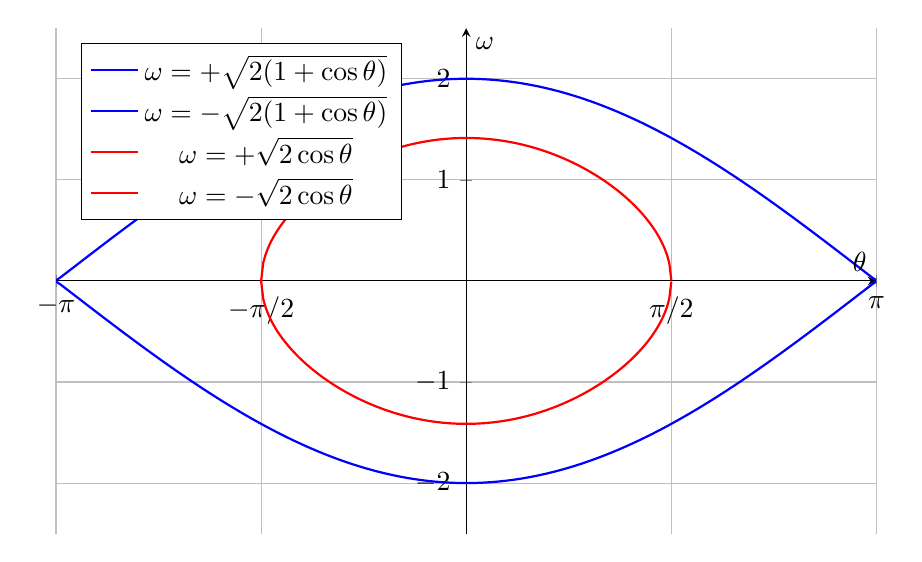
\begin{tikzpicture}
\begin{axis}[
    width=12cm,
    height=8cm,
    xlabel={$\theta$},
    ylabel={$\omega$},
    xmin=-pi, xmax=pi,
    ymin=-2.5, ymax=2.5,
    xtick={-pi, -pi/2, 0, pi/2, pi},
    xticklabels={$-\pi$, $-\pi/2$, $0$, $\pi/2$, $\pi$},
    grid=major,
    legend pos=north west,
    axis lines=center,
    samples=200,
    domain=-pi:pi,
]

% Upper branch: omega = sqrt(2(1+cos(theta)))
\addplot[blue, thick] {sqrt(2*(1+cos(deg(x))))};
\addlegendentry{$\omega=+\sqrt{2(1+\cos\theta)}$}

% Lower branch: omega = -sqrt(2(1+cos(theta)))
\addplot[blue, thick] {-sqrt(2*(1+cos(deg(x))))};
\addlegendentry{$\omega=-\sqrt{2(1+\cos\theta)}$}

% Upper branch: omega = sqrt(2*cos(theta)) for |theta| < pi/2
\addplot[red, thick, domain=-pi/2:pi/2] {sqrt(2*cos(deg(x)))};
\addlegendentry{$\omega=+\sqrt{2\cos\theta}$}

% Lower branch: omega = -sqrt(2*cos(theta)) for |theta| < pi/2
\addplot[red, thick, domain=-pi/2:pi/2] {-sqrt(2*cos(deg(x)))};
\addlegendentry{$\omega=-\sqrt{2\cos\theta}$}

\end{axis}
\end{tikzpicture}
\caption{Phase space trajectories}
\end{figure}

\subsection{Part (c)}

Given that $\theta$ is on the circle $S^1$, the length of our cylinder is $\omega$. What the problem is asking is whether there are any closed orbits with $\theta$ strictly contained within $S^1$ (in other words, there is no wrap around from $+\pi$ to $-\pi$ or vice versa). The hint to use Bendixson's criterion is suggesting that we use Bendixson's criterion to rule out periodic orbits, thus making it impossible that there are closed orbits, and hence, closed orbits that encircle the `phase cylinder'. Note that Bendixson's criterion only applies for simply connected sets in our phase plane; however, this is requirement is met with the problem statement asking whether there are any closed orbits with $\theta$ contained within $S^1$. By focusing strictly within $S^1$, we are constraining ourselves to only look at regions that can be described with simply connected sets.

Computing $\nabla\cdot(f,g)$, we have 
\begin{align*}
  \nabla\cdot(f,g)&=\partial_\theta \omega+\partial_\omega\left(\beta-\delta\omega-\sin\theta\right)\\
  &=0-\delta\\
  &=-\delta
\end{align*}
Via Bendixson's criterion, this system can only have periodic orbits if $\nabla\cdot(f,g)$ equals zero or changes sign. In our case, $\nabla\cdot(f,g)$ can only equal zero if $\delta=0$. Hence, the system can have closed orbits that do not encircle the `phase cylinder' only if $\delta=0$.

Moreover, we found such orbits in part (b) of this problem.

\subsection{Part (d)}

In line with the hint, our approach to the problem is to define a trapping region on $\omega$ and then use Poincaré-Bendixson theorem to argue there is a closed orbit. The trapping region on $\omega$ can be found by realizing the the $-\sin\theta$ term in $\dot{\omega}$ is bound by $+1$ and $-1$. To find an upper bound such that $0>\dot{\omega}$, we can set $\theta$ such that $-\sin\theta=+1$, and then write
\[0>\dot{\omega}=\beta-\delta\omega+1\]
where it implies that
\[ \omega>\frac{\beta+1}{\delta} \]
Hence if we have an initial $\omega(0)$ greater than $\frac{\beta+1}{\delta}$, regardless of $\theta$, $\dot{\omega}$ is negative. For the lower bound, we need to find $\dot{omega}>0$, hence we set $\theta$ such that $-\sin\theta=-1$ and write
\[
\beta-\delta\omega-1=\dot{\omega}>0
\]
where we have
\[
\frac{\beta-1}{\delta} > \omega
\]
Hence if we have an initial $\omega(0)$ less than $\frac{\beta-1}{\delta}$, regardless of $\theta$, $\dot{\omega}$ is positive. Therefore, we have a trapping region 
\[ U=\left\{(\theta,\omega): \omega\in\left[\frac{\beta-1}{\delta} - \epsilon, \frac{\beta+1}{\delta}+\epsilon \right] \right\}
\]
for some $\epsilon>0$. Also note that $U$ wraps around that phase cylinder in the $\theta$ direction, hence it is a compact set.

By setting $\beta>1$, part (a) tells us that there are no fixed points in the system; hence, there would be no fixed points in $U$. Therefore, applying Poincaré-Bendixson theorem, we can deduce that there must be a closed orbit in $U$.

\end{solution}

\clearpage

\begin{problem}
We consider the ``rabbit vs. sheep'' system described by the following equations:
\begin{align*}
  \dot{x}&=x(3-x-2y)\\
  \dot{y}&=y(2-x-y),
\end{align*}
where $x$ represents the population of rabbits, and $y$ represents the population of sheep.
\begin{itemize}
  \item[(a)] Find all the equilibria of the system, and for each determine its index.
  \item[(b)] Show that it is impossible to have a closed orbit for the system (index theory will help but you will need something else to rule out all possible closed orbit).
\end{itemize}

\end{problem}

\begin{solution}
\section{Problem 2}
\subsection{Part (a)}

Finding the fixed points, we set the system to zero to get 
\begin{align*}
  0&=\dot{x}=x(3-x-2y)\\
  0&=\dot{y}=y(2-x-y)
\end{align*}
Clearly, fixed points arise when $x=0$ and $y=0$. In particular, a fixed point at the origin $(0,0)$, when $x=0$ we have 
\[0=2-0-y\implies y=2\]
giving a fixed point at $(0,2)$, and when $y=0$ we have 
\[0=3-x-2(0)\implies x=3\]
giving a fixed point at $(3,0)$. When $x\neq0$ and $y\neq0$, we can write 
\begin{align*}
  0&=3-x-2y\\
  0&=2-x-y
\end{align*}
and then 
\begin{gather*}
  3-x-2y=2-x-y\\
  -y=-1\\
  y=1
\end{gather*}
Plugging $y=1$ into $0=2-x-y$, we get a fixed point at $(1,1)$.

Hence, all our fixed points are 
\begin{itemize}
  \item $(0,0)$
  \item $(0,2)$
  \item $(3,0)$
  \item $(1,1)$
\end{itemize}
Now let's linearize. We can generically write the Jacobian as 
\[ J_f(x,y) = \begin{bmatrix}
3-2x-2y & -2x \\
-y & 2-x-2y
\end{bmatrix} \]
Now let's compute the eigenvalues for each Jacobian around each fixed point.

For $(0,0)$, we have 
\[ J_f(0,0) = \begin{bmatrix}
3 & 0\\
0 & 2
\end{bmatrix} \]
where the eigenvalues, found via the diagonal, are $\lambda_0=3$ and $\lambda_1=2$. Hence, this is an unstable fixed point (source), with an index of $+1$.

For $(0,2)$, we have 
\[ J_f(0,2) = \begin{bmatrix}
-1 & 0\\
-2 & -2
\end{bmatrix} \]
where the eigenvalues, found via the diagonal, are $\lambda_0=-1$ and $\lambda_1=-2$. Hence, this is a stable fixed point (sink), with an index of $+1$.

For $(3,0)$, we have 
\[ J_f(3,0) = \begin{bmatrix}
-3 & -6\\
0 & -1
\end{bmatrix} \]
where the eigenvalues, found via the diagonal, are $\lambda_0=-3$ and $\lambda_1=-1$. Hence, this is a stable fixed point (sink), with an index of $+1$.

For $(1,1)$, we have 
\[ J_f(3,0) = \begin{bmatrix}
-1 & -2\\
-1 & -1
\end{bmatrix} \]
where the eigenvalues, found via SymPy, are $\lambda_{0,1}=-1\pm\sqrt{2}$, where $-1+\sqrt{2}$ is positive. Hence, there is are positive and negative eigenvalues, implying the fixed point is a saddle, with an index of $-1$.

\subsection{Part (b)}

To start, let's note the following corollary on page 51 of the textbook:

\noindent
\textbf{Corollary 1.8.5.} \textit{Inside any closed orbit $\gamma$ there must be at least one fixed point. If all the fixed points within $\gamma$ are hyperbolic, then there must be an odd number, $2n+1$, of which $n$ are saddles and $n+1$ either sinks or sources.}

Looking at our system, all four fixed points are hyperbolic. Hence, if there is any closed orbit, it must either just contain $(0,2),(3,0),(0,0)$ or contain the one saddle at $(1,1)$ and 
\begin{itemize}
  \item the two sinks $(0,2),(3,0)$,
  \item the $(0,2)$ sink and the $(0,0)$ source,
  \item or the $(3,0)$ sink and the $(0,0)$ source.
\end{itemize}

What's nice about our sinks and sources is that they all lie along the x or y axis. From our system of equations, notice that if $x=0$, then it follows that 
\begin{align*}
  \dot{x}&=0\\
  \dot{y}&=y(2-y),
\end{align*}
which means that trajectories starting on the y-axis stay on the y-axis, implying that the y-axis is an invariant set. Also notice that if $y=0$, then it follows that 
\begin{align*}
  \dot{x}&=x(3-x)\\
  \dot{y}&=0,
\end{align*}
which means that trajectories starting on the x-axis stay on the x-axis, implying that the x-axis is an invariant set.

Hence, if a closed orbit were to encompass one of our sinks or sources, the closed orbit would have to cross the x or y axis, both being invariant sets. This is impossible since we would violate the existence and uniqueness of solutions at some point $p$ where closed orbit intersects the axis since $p$ would belong to two distinct trajectories. Therefore, any closed orbit in the system cannot contain $(0,2),(3,0),(0,0)$, and via our reasoning with index theory, it is impossible to have a closed orbit for the system.

\end{solution}

\clearpage

\begin{problem}
Consider the following second-order, periodically forced, differential equation:
\begin{equation}\label{eq:prob_3}
  \ddot{x}+\delta\dot{x}+f(x)=\gamma\cos\left(\omega t\right).
\end{equation}
\begin{itemize}
  \item[(a)] Letting $f(x)=x$ and fixing $\omega=1,\delta>0,\gamma>0$, show that there exists a $2\pi$-periodic solution to (\ref{eq:prob_3}).
  \item[(b)] Construct a Poincaré map that takes $(x(0),\dot{x}(0))$ to $(x(T),\dot{x}(T))$, where $T=2\pi/\omega$ is the forcing period, and use this map to investigate the stability of the periodic orbit you found in part (a).
  \item[(c)] Now let $f(x)=\sin x$, and fix $\delta=\gamma=0$. Show that (\ref{eq:prob_3}) possess a homoclinic orbit $q^0(t)$ to a hyperbolic saddle point $p_0$. [\textit{Hint:} Recognize that the system is Hamiltonian and use the conserved quantity.]
  \item[(d)] Now let $\delta,\gamma>0$, and consider how this perturbation might affect the fixed point $p_0$ and the homoclinic orbit. Under the periodic forcing, the fixed point $p_0$ is perturbed to a \textit{periodic orbit} (of saddle type). This periodic orbit is a fixed point of the Poincaré map that takes $(x(0),\dot{x}(0))$ to $(x(T),\dot{x}(T))$. Find an approximation to this periodic orbit numerically (e.g., in Python or Matlab), by constructing a numerical approximation to the Poincaré map, and using a numerical root finder to find a fixed point close to $p_0$.
  \item[(e)] Now investigate (numerically) what happens to the homoclinic orbit $q^0(t)$, for $\delta,\gamma>0$. Do your best to numerically approximate the stable and unstable manifolds of the fixed point you found in the previous part, for some values of $\delta,\gamma,\omega$: for instance, place a bunch of points along the stable and unstable eigenspaces, and iterate them forward or backward using your Poincaré map. Can you find values for which the stable and unstable manifolds have transversal intersections? If so, can you find something resembling ``chaotic'' behavior?\newline [\textit{Hint:} In the coming weeks, we will learn a technique for predicting when such transversal intersections occur, and if $\delta,\gamma\ll 1$, this theory predicts that transversal intersections occur when \[\frac{\gamma}{\delta}>\frac{4}{\pi}\cosh\left(\frac{\pi\omega}{2}\right).\] Let this guide your numerical explorations.]
\end{itemize}

\end{problem}

\begin{solution}

\section{Problem 3}

\subsection{Part (a)}

To show that a $2\pi$-periodic solution to (\ref{eq:prob_3}) exists, let's use the method of undetermined coefficients where we guess that $x(t)$ is 
\[ x(t)=A\cos\left( t\right) + B\sin\left( t\right) \]
and then we can compute the following values 
\begin{align*}
  \dot{x}&=-A\sin\left( t\right)+B\cos\left( t\right)\\
  \ddot{x}&=-A\cos\left( t\right) - B\sin\left( t\right)
\end{align*}
Now we can through our values into the following equation 
\[\ddot{x}+\delta\dot{x}+x=\gamma\cos\left( t\right)\]
to get 
\begin{align*}
  \gamma\cos\left( t\right)&=-A\cos\left( t\right) - B\sin\left( t\right)+\delta\left(-A\sin\left( t\right)+B\cos\left( t\right)\right)+A\cos\left( t\right) + B\sin\left( t\right)\\
  &=-A\delta\sin(t)+B\delta\cos(t)
\end{align*}
where $A=0$ and $B=\frac{\gamma}{\delta}$. Hence our $2\pi$-periodic solution to (\ref{eq:prob_3}) is 
\[x(t)=\frac{\gamma}{\delta}\sin(t) \]

\subsection{Part (b)}

First, let's reparameterize our system such that it is an autonomous system of ODEs:
\begin{align*}
  \dot{x}&=y\\
  \dot{y}&=-\delta y -f(x)+\gamma\cos\psi\\
  \dot{\psi}&=\omega
\end{align*}
Now let's look at the section 
\[
\Sigma=\left\{\left(x,y,\psi\right) : \psi=0\, \mod 2\pi  \right\}
\]
This is convenient because our system becomes 
\begin{align*}
  \dot{x}&=y\\
  \dot{y}&=-\delta y -f(x)+\gamma\\
\end{align*}
where we could linearize around some closed orbit $\zeta$ to get 
\[ \dot{\xi}= D_xf(\zeta)\cdot \xi \]
Here, $D_xf(\zeta)$ is the Jacobian
\[ J_f(x,y) = \begin{bmatrix}
\frac{\partial f_1}{\partial x} & \frac{\partial f_1}{\partial y} \\
\frac{\partial f_2}{\partial x} & \frac{\partial f_2}{\partial y} 
\end{bmatrix} \]
with the quantities being 
\begin{gather*}
  \frac{\partial f_1}{\partial x}=0\\
  \frac{\partial f_1}{\partial y}=1\\
  \frac{\partial f_2}{\partial x}=-f'(x)\\
  \frac{\partial f_2}{\partial y}=-\delta
\end{gather*}
Putting it all together, the Jacobian is
\[ J_f(x,y) = \begin{bmatrix}
0 & 1 \\
-f'(x) & -\delta
\end{bmatrix} \]
and our Poincaré map is given by Floquet theory by solving $\dot{\xi}= D_xf(\zeta)\cdot \xi$ to get 
\[\xi(t)=\Phi(t)\xi(0)\]
where $\Phi(t)$ is the fundamental solution matrix.

Now looking at the orbit in part (a), we have $-f'(x)=-1$. Thus our Jacobian at the stable orbit is 
\[ A(t)=J_f(x(0),y(0)) = \begin{bmatrix}
0 & 1 \\
-1 & -\delta
\end{bmatrix} \]
where $x(0),y(0)$ is 
\[ x(0)=\frac{\gamma}{\delta}\sin 0=0 \]
and 
\[ y(0)=\dot{x}(0)=\frac{\gamma}{\delta}\cos 0 =\frac{\gamma}{\delta}\]
This is nice because our Jacobian $A(t)$ is time-independent, hence just $A$, and by finding Floquet exponents, we can reason about the stability of the Poincaré map. Evaluating our eigenvalues and eigenvectors of the Jacobian via SymPy, we have 
\[
\left[ \left( \lambda_0 = - \frac{\delta}{2} - \frac{\sqrt{\delta^2-4}}{2}, \  v_0= \left[\begin{matrix}\lambda_1\\1\end{matrix}\right]\right), \  \left(\lambda_1= - \frac{\delta}{2} + \frac{\sqrt{\delta^2-4}}{2}, \  v_1= \left[\begin{matrix}\lambda_0\\1\end{matrix}\right]\right)\right]
\]
where our eigenvalues $\lambda_0,\lambda_1$ always have a negative real part since $\delta>0$, $\delta<2$ implies that $\sqrt{\delta^2-4}$ is imaginary, and for $\delta>2$ we have $\delta>\sqrt{\delta^2-4}$, implying $\lambda_1$ is negative.

To get the Poincaré map, we solve $\dot{\xi}= D_xf(\zeta)\cdot \xi$ to get 
\[\xi(T)=e^{TA}\xi(0) \]
where our Floquet exponents $\lambda_0,\lambda_1$ of $A$ become eigenvalues $e^{\lambda_0T},e^{\lambda_1T}$ of the Poincaré map. Hence, because $\lambda_0,\lambda_1$ both had negative real parts, $e^{\lambda_0T},e^{\lambda_1T}$ are both less than one, implying that the map is stable around our closed orbit.

Note that even if $\lambda$ is complex with a negative real part, we can write 
\[ e^{\lambda T}=e^{T\mathrm{Re} \lambda+i\,T\mathrm{Im} \lambda}=e^{T\mathrm{Re} \lambda}e^{i\,T\mathrm{Im} \lambda}=e^{T\mathrm{Re} \lambda}\left(\cos\left(T\mathrm{Im} \lambda\right)+i\,\sin\left(T\mathrm{Im} \lambda\right)\right)\]
which will have a length less than 1. Hence, even if $\lambda$ is complex with a negative real part, the Poincaré map is still stable.

\subsection{Part (c)}

Now letting $f(x)=\sin x$ and fixing $\delta=\gamma=0$, our system is 
\[
\ddot{x}+\sin x =0
\]
and via reparameterizing, we have 
\begin{align*}
  \dot{x}&=y\\
  \dot{y}&=-\sin x
\end{align*}

First, let's find the fixed points to show that a hyperbolic saddle point exists. We can write 
\begin{align*}
  0&=\dot{x}=y\\
  0&=\dot{y}=-\sin x
\end{align*}
where it becomes clear that our fixed points are $(\pm n\pi,0)$ for $n\in\mathbb{Z}$. To linearize, we can compute the Jacobian 
\[ J_f(x,y) = \begin{bmatrix}
\frac{\partial f_1}{\partial x} & \frac{\partial f_1}{\partial y} \\
\frac{\partial f_2}{\partial x} & \frac{\partial f_2}{\partial y} 
\end{bmatrix} \]
with the quatities being 
\begin{gather*}
  \frac{\partial f_1}{\partial x}=0\\
  \frac{\partial f_1}{\partial y}=1\\
  \frac{\partial f_2}{\partial x}=-\cos x\\
  \frac{\partial f_2}{\partial y}=0
\end{gather*}
Now we can compute our linearized matrices 
\begin{gather*}
  Df(0,0)=\begin{bmatrix}
    0 & 1\\
    -1 & 0
  \end{bmatrix}\\
  Df(+\pi,0)=\begin{bmatrix}
    0 & 1\\
    1 & 0
  \end{bmatrix}
\end{gather*}

Notice that I only calculated the Jacobian matrices for $0,+\pi$ since more multiples of $\pi$ will be one of these two matrices. 

Calculating the eigenvalues and eigenvectors, for equilibria $(0,0)$ and corresponding $2\pi$ multiples, we have 
\[\left[ \left( \lambda=- i, \  v= \left[\begin{matrix}i\\1\end{matrix}\right]\right), \  \left( \lambda=i, \  v=\left[\begin{matrix}- i\\1\end{matrix}\right]\right)\right]
\]
implying that linearization tells us nothing since we have 0 real part to our eigenvalues.

Calculating the eigenvalues and eigenvectors, for equilibria $(+\pi,0)$ and corresponding $2\pi$ multiples, we have 
\[\left[ \left( \lambda=-1, \  v=\left[\begin{matrix}-1\\1\end{matrix}\right]\right), \  \left( \lambda=1, \  v= \left[\begin{matrix}1\\1\end{matrix}\right]\right)\right]\] 
where we have an unstable fixed point due to the positive eigenvalue. Specifically, it is a saddle.

Given the hint, we can recognize that the system is Hamiltonian, and go looking for such Hamiltonian. We start by solving for $\partial H/\partial y$
\begin{gather*}
  \frac{\partial H}{\partial y}=y\\
  \partial H = y\partial y\\
  \int \partial H = \int y\partial y\\
  H(x,y) = \frac{y^2}{2}+f(x)
\end{gather*}
and by solving for $\partial H/\partial x$, we have 
\begin{gather*}
  -\frac{\partial H}{\partial x}=-\sin x\\
  \partial H = \sin x \,\partial x\\
  \int \partial H = \int \sin x \,\partial x\\
  H(x,y) = -\cos x +g(y)
\end{gather*}
Putting it all together, we have 
\[ H(x,y) = \frac{y^2}{2} - \cos x \]

Plugging in our saddle point $(\pi,0)$ to our Hamiltonian, we have 
\[
H(\pi,0)=\frac{0^2}{2}-\cos\pi=1
\]
Now to show that there is a homoclinic orbit $q^0(t)$ to the hyperbolic saddle point $p_0=(\pi,0)$, we can use the Hamiltonian to get an expression for y in terms of x, and then we can show that this expression goes to $p_0$. Hence, we can write 
\begin{gather*}
  \frac{y^2}{2} - \cos x=1\\
  y^2=2\left(\cos x + 1\right)\\
  y=\pm\sqrt{2\left(\cos x + 1\right)}
\end{gather*}

Given that the system is $2\pi$-periodic in $x$, our saddle points at $(\pi,0)$ and $(-\pi,0)$ are really the same saddle point. This makes sense given that this system is a driven pendulum. Hence, if we start at $(\pi,0)$, and travel along either $+\sqrt{2(\cos x + 1)}$ or $-\sqrt{2(\cos x + 1)}$, we will make it back to $(-\pi,0)$, the same saddle point. Hence, we have a homoclinic orbit.

Note that our curves $y=\pm\sqrt{2\left(\cos x + 1\right)}$ don't intersect with our only other fixed point at $(0,0)$. This is because our Hamiltonian evaluated at $(0,0)$ is $H(0,0)=-1$; therefore it lies on a different level set entirely.

\subsection{Part (d)}

Note that for parts (d) and (e), I did them both simultaneously, so it's relevant to note that I computed some potential values for $\gamma,\delta$ via the hint. Let's just say $\delta=0.01$ and then compute what $\gamma$ might be. Hence we can write 
\[\gamma > 0.01\left(\frac{4}{\pi}\cosh\left(\frac{\pi\omega}{2}\right)\right)=0.03195 \]
and we could set $\gamma=0.2$.

With a generous use of generative AI, I made the following code:
\begin{lstlisting}
import numpy as np
import matplotlib.pyplot as plt 

from scipy.integrate import solve_ivp
from scipy import optimize


def driven_pendulum(t, z):
    delta, gamma, omega = 0.01, 0.2, 1.0
    x, y = z
    dx = y
    dy = -delta*y - np.sin(x) + gamma*np.cos(omega*t)
    return [dx,dy]

def residual(y0):
    t_span = (0, 2*np.pi)
    sol = solve_ivp(
        driven_pendulum, t_span, y0, 
        t_eval=np.linspace(0, 2*np.pi, 300)
    )
    return [sol.y[0][-1] - y0[0], sol.y[1][-1] - y0[1]]

guess = [1.0, 0.0]
result = optimize.root(residual, guess, method='hybr')
print(f"Success: {result.success}")
print(f"Periodic orbit initial condition: {result.x}")

t_span = (0, 2*np.pi)
y0 = result.x
sol = solve_ivp(
  driven_pendulum, t_span, y0, 
  t_eval=np.linspace(0, 2*np.pi, 300)
)
\end{lstlisting}

The identified orbit is indeed a periodic orbit of saddle type, with the eigenvalues being 
\[\lambda_0=5.15278292e+02,\qquad\lambda_1=-1.74208404e-02\]

\begin{figure}[h]
\caption{Periodic orbit}
\centering
\includegraphics[width=0.75\textwidth]{problem_3/problem_3_d.png}
\end{figure}

\subsection{Part (e)}

My approach to this problem was to create a Poincaré map from part (d), approximate the Jacobian of the Poincaré map, select two points slightly along the stable and unstable eigenspaces, and iterate them backward and forward respectively.

With a generous use of generative AI, I made the following code:
\begin{lstlisting}
def poincare_map(y0):
    t_span = (0, 2*np.pi)
    sol = solve_ivp(driven_pendulum, t_span, y0, dense_output=True)
    return sol.y[:, -1]

def jacobian_finite_diff(y0, diff=1e-6):
    J = np.zeros((2, 2))
    yT = poincare_map(y0)
    
    for i in range(2):
        y_perturbed = y0.copy()
        y_perturbed[i] += diff
        yT_perturbed = poincare_map(y_perturbed)
        J[:, i] = (yT_perturbed - yT) / diff
    
    return J

# Approximate stable and unstable eigenspaces
jacobian = jacobian_finite_diff(y0)
eigen_comps = np.linalg.eig(jacobian)

eps = 0.0001

# Iterate a point on the unstable manifold forward
y_unstable = y0 + eps*eigen_comps.eigenvectors[:,0]
sol_unstable = solve_ivp(
    driven_pendulum, (0, 2*np.pi), y_unstable, 
    t_eval=np.linspace(0, 2*np.pi, 300)
)

# Iterate a point on the stable manifold backward
y_stable = y0 + eps*eigen_comps.eigenvectors[:,1]

sol_stable = solve_ivp(
    driven_pendulum, (0, -2*np.pi), y_stable, 
    t_eval=np.linspace(0, -2*np.pi, 300)
)
\end{lstlisting}

\begin{figure}[ht]
\caption{Transversal intersection}
\centering
\includegraphics[width=0.75\textwidth]{problem_3/problem_3_e_manifolds.png}
\end{figure}

Simulating a few trajectories slightly perturbed from $p_0$, we get Figure 4 demonstrating chaotic behavior. Note that trajectories intersect because we are not plotting $\dot{x}$.

\begin{figure}[ht]
\caption{Trajectories demonstrating chaos}
\centering
\includegraphics[width=0.75\textwidth]{problem_3/spacetime_cylinder.png}
\end{figure}

\end{solution}


\end{document}